\chapter{Comparative between CPU and GPU}
\label{ch::chapter5}

\vspace{-1cm}


\section{Speedup (GPU / CPU)}
\label{sec:cpu_gpu_speedup}

This section condenses the comparison to two core views:
(A) FP32 MxM vs.\ MxV speedup, and
(B) FP64 MxM vs.\ MxV speedup.
Here, when we refer to speedup, we mean GPU GFLOPS divided by CPU (multi-thread) GFLOPS.

\subsubsection*{(A) FP32: \textnormal{MxM} vs.\ \textnormal{MxV} Speedup}

In FP32, both MxM and MxV deliver a clear advantage for GPU over CPU. The effect is much stronger for MxM because it is compute-bound, while MxV also improves but plateaus lower due to its bandwidth-bound nature.

\vspace{-1em}

\begin{figure}[H]\centering
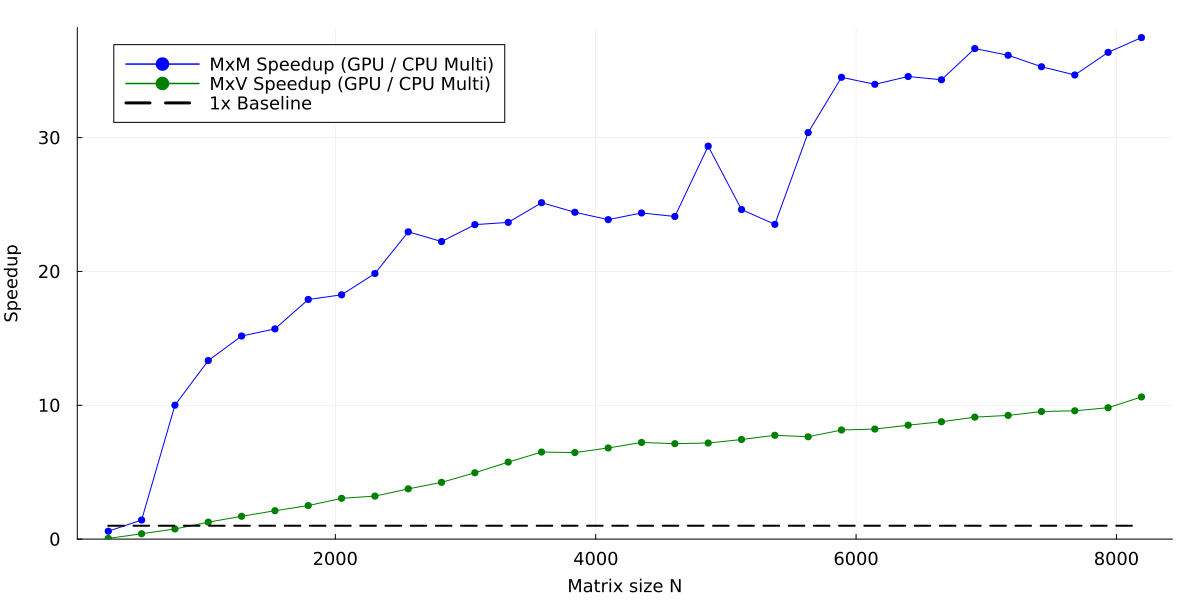
\includegraphics[width=\textwidth]{figures/5_cpu_vs_gpu/Float32_GFLOPS_speedup.png}
\caption{\textbf{FP32 speedup (GPU/CPU): MxM vs.\ MxV.} MxM rapidly enters a high speedup regime as the GPU saturates compute; MxV remains bandwidth-limited and achieves a smaller but noticeable, flatter speedup. We can clearly assume the superiority of GPUs against CPUs for large problem sizes, in both MxM and MxV operations.}
\label{fig:speedup_fp32_ab}
\end{figure}

It is important to clarify that for very large sizes, the speedup widens further mostly because the CPU side falls off (all-core turbo drops, memory pressure rises, thermal throttling and BLAS strategies become less favorable) so CPU GFLOPS decline while the GPU holds steady.

Even we cannot see where the plateau for MxM exactly begins, do not expect the speedup to keep increasing indefinitely with $N$ as this was caused by the GPU's ability to maintain high throughput because of better handling in thermals and libraries, compared to the CPU.

\vspace{2em}

\subsubsection*{(B) FP64: \textnormal{MxM} vs.\ \textnormal{MxV} Speedup}
In FP64, consumer GPUs throttle floating-point throughput, so MxM speedup is much lower than in FP32 even at large $N$: the kernel remains compute-bound, but the architectural FP64 cap limits the attainable advantage over the CPU.

By contrast, MxV is still memory-bound and can exploit the GPU’s much higher memory bandwidth. As a result, its FP64 speedup becomes larger than MxM’s (the gap even flips, having a higher speedup on MxV than MxM).

This is the key takeaway for FP64: compute throttling shrinks MxM’s headroom, while MxV continues to benefit from fast GDDR, yielding a comparatively healthy speedup.

\begin{figure}[H]\centering
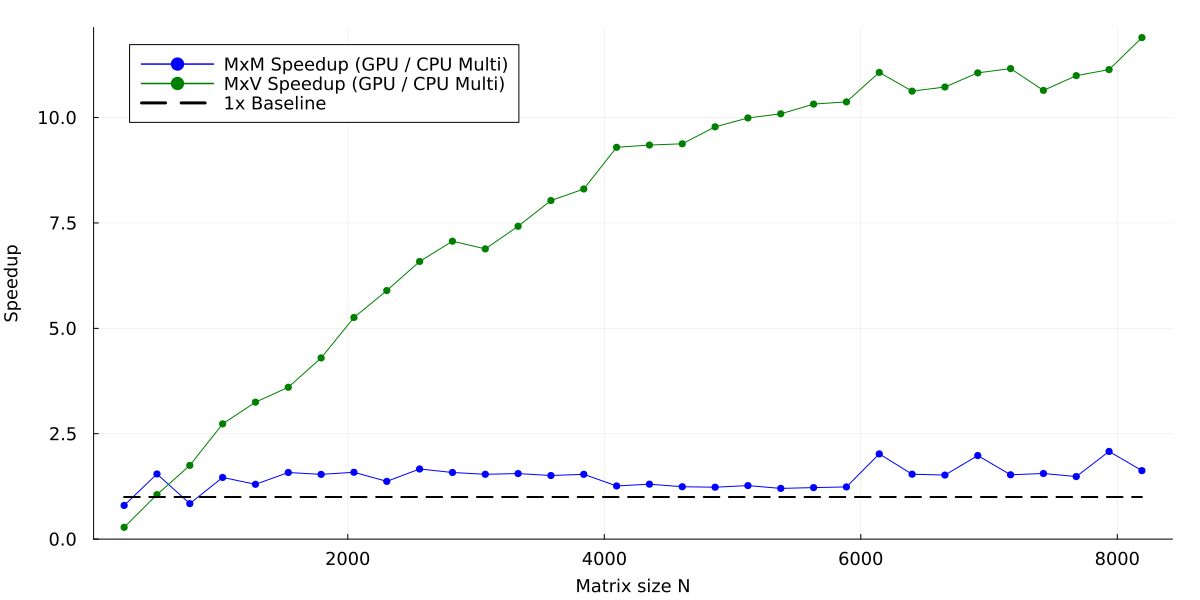
\includegraphics[width=\textwidth]{figures/5_cpu_vs_gpu/Float64_GFLOPS_speedup.png}
\caption{\textbf{FP64 speedup (GPU/CPU): MxM vs.\ MxV.} MxM rapidly enters a high speedup regime as the GPU saturates compute; MxV remains bandwidth-limited and achieves a smaller, flatter speedup.}
\label{fig:speedup_fp64_ab}
\end{figure}